\chapter{练习题答案}
\label{cha:answers}
\fancyhead[OL]{\bfseries\nouppercase\rightmark}
\setcounter{section}{-1}

本书每一章节的末尾都会有数道练习题,其中一些需要你进行实际操作,另一些则需要你动脑思考。这里我们列出那些需要动脑思考的练习题的答案。

\section{\nameref{cha:first-things-first}}

\begin{enumerate}
  \item $1\,\mathrm{GB}=1024^2\,\mathrm{KB}$。进一步计算得到 $1\,\mathrm{GB}=1024^3\,\text{字节}$,那么可以存储 $\dfrac{1024^3}{2}$ 即大约 5 亿个汉字。
  \item 「1000 进位」下,64 GB 是 $64\times1000^3\,\text{字节}$,这么多字节按照「1024 进位」则是 $\dfrac{64\times1000^3}{1024^3}\,\mathrm{GB}\approx59.6\,\mathrm{GB}$。这意味着你去购买的「64 GB」U 盘,在电脑中显示的总空间应该在 59 GB 附近。
  \item 这些快捷键的功能应该如下:
  \begin{enumerate}
    \item 可以截屏。按下这个快捷键后进行框选截屏,截屏后图像保存在剪切板中。
    \item 可以打开「任务管理器」。
    \item 可以迅速返回桌面。
  \end{enumerate}
  \item 略。
\end{enumerate}

\section{\nameref{cha:computer-and-its-components}}

略。

\section{\nameref{cha:file-and-file-management}}

略。

\section{\nameref{cha:software-installation}}

\begin{enumerate}
  \item 灰色的【本地下载】按钮,如图\autoref{fig:SoftInst_1}。
    \begin{figure}[htb!]
      \centering
      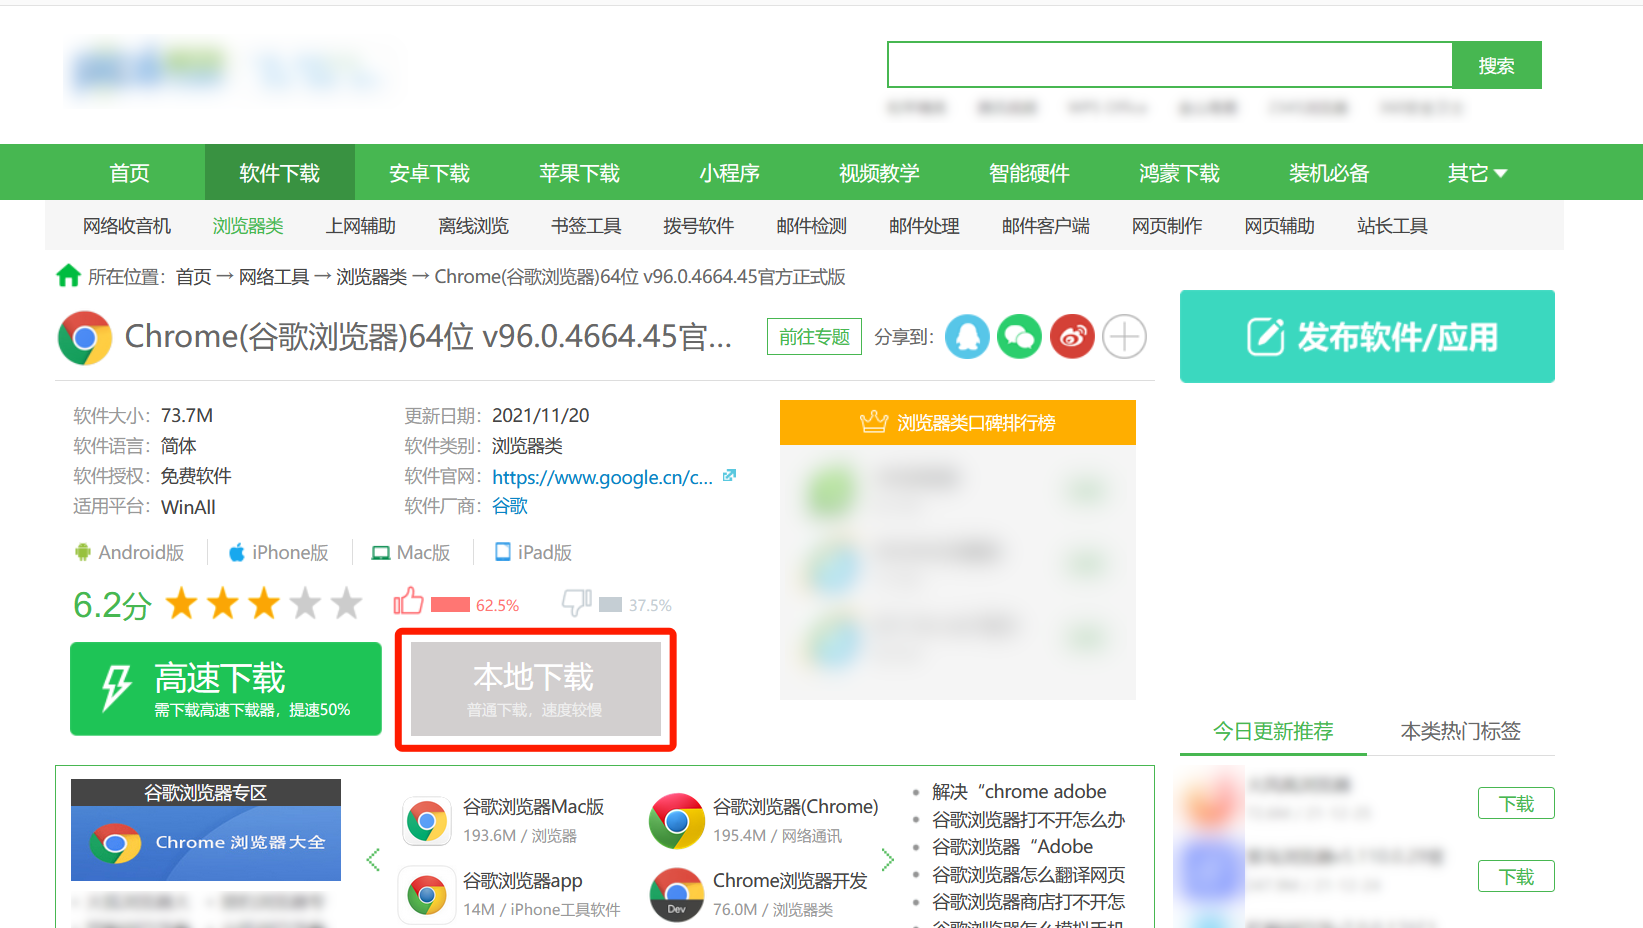
\includegraphics[width=.8\textwidth]{assets/appendix/SoftInst_1.png}
      \caption{【本地下载】}
      \label{fig:SoftInst_1}
    \end{figure}
  \item 「普通下载地址」下方的四个「✕✕远程下载」按钮。
  \item 取消勾选「使用搜狗软件助手下载软件」,然后寻找「普通下载」按钮。
  \item 5 个。
  \item C 项。
  \item B 项。A 项将 Steam 这种大型游戏平台安装在了 C 盘;C 项软件安装路径中有中文;D 项直接把软件装在桌面中的某个文件夹里,而且路径中还有中文。
  \item 不可以。
\end{enumerate}

\section{\nameref{cha:basic-maintenance}}

\begin{enumerate}
  \item 左方没有高亮的【继续卸载】按钮。
  \item 左方没有高亮的【确认卸载】按钮。
  \item 右下方的【残忍卸载】小字。
    \begin{figure}[htb!]
      \centering
      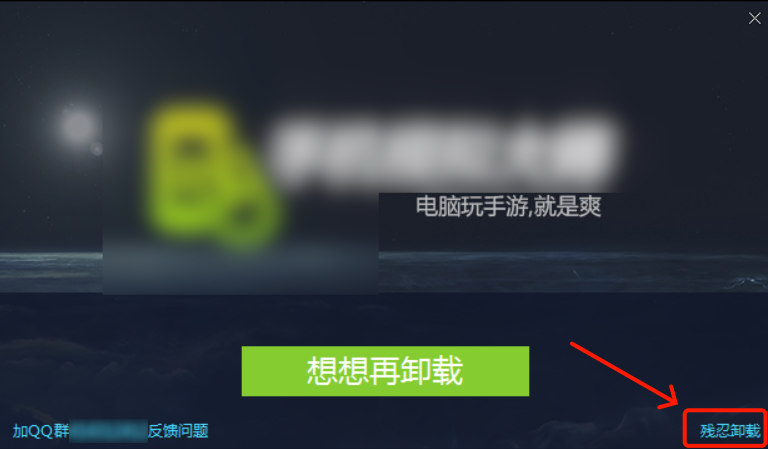
\includegraphics[width=.55\textwidth]{assets/appendix/BasicMaint_3.png}
      \caption{【残忍卸载】四个小字}
      \label{fig:BasicMaint_3}
    \end{figure}
  \item 先点选【卸载】,然后寻找「残忍卸载」之类的按钮。
    \begin{figure}[htb!]
      \centering
      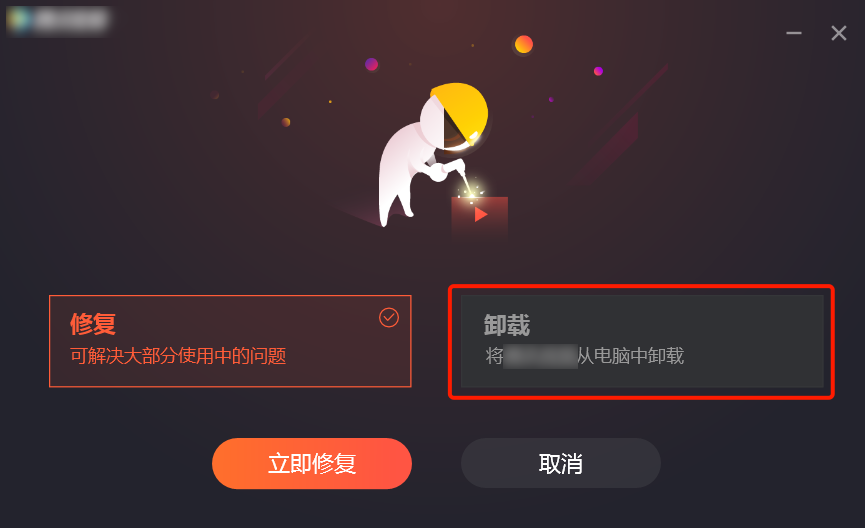
\includegraphics[width=.55\textwidth]{assets/appendix/BasicMaint_4.png}
      \caption{点击【卸载】}
      \label{fig:BasicMaint_4}
    \end{figure}
  \item 略。
\end{enumerate}

\section{\nameref{cha:how-to-find-solutions}}

\begin{enumerate}
  \item 使用下面这样的搜索语句应该更容易帮助你找到答案:
    \begin{quoting}
      pr 加速渲染器错误 无法生成帧 1609629690
    \end{quoting}
    虽然错误代码前面有个负号,但搜索时可不能添加,因为它可能触发搜索引擎的「排除关键词」过滤规则。
  \item 弹出这个说明这个软件需要「.Net Framework 3.5」这个东西,而你的电脑没有。既然系统给出了解决方案,那么我们直接点击【下载并安装此功能】就可以了。
  \item 弹出这个说明这个软件需要某个组件,而我们的电脑缺少它。用下面的搜索语句在网络上搜索:
    \begin{quoting}
      api-ms-win-crt-runtime-l1-1-0.dll 缺失
    \end{quoting}
    查阅相关文章,容易得知是缺失「VC++ 运行库」造成的。上网搜索下载相应的组件安装即可。
\end{enumerate}

\section{\nameref{cha:shortcut-keys}}

略。

\section{\nameref{cha:office-and-wps}}

略。

\section{\nameref{cha:browsers-and-how-to-choose}}

\begin{enumerate}
  \item 略。
  \item 略。
  \item 不是。和杀毒软件一样,当你安装了多个浏览器时,它们可能会因为争着成为你的「默认浏览器」而「打架」。
\end{enumerate}

\section{\nameref{cha:mail-and-instant-messaging}}

\begin{enumerate}
  \item 略。
  \item 可以查看发信人的邮箱地址,如果域名不是各大银行的官网域名(比如,建行的 \texttt{ccb.com},平安银行的 \texttt{pingan.com}),就说明这邮件很可能是假的。
  \item 略。
\end{enumerate}

\section{\nameref{cha:archive-formats-and-tools}}

略。

\section{\nameref{cha:tools-software}}

略。

\section{\nameref{cha:how-to-find-tutorials}}

略。

\section{\nameref{cha:screens-and-their-secrets}}

\begin{enumerate}
  \item 略。
  \item 提示:利用正文中的公式计算即可。
  \item 略。
\end{enumerate}

\section{\nameref{cha:user-and-ms-account}}

\begin{enumerate}
  \item 略。
  \item 略。
  \item 因为 Administrator 的权限太大,打开任何程序都会赋予它很高的权限,而且又没有提示,因此恶意软件可以为所欲为而不被我们知晓;另外,因我们乱改系统设置和文件造成系统损坏的概率也会直线上升。
\end{enumerate}

\section{\nameref{cha:recover-from-bsod}}

\begin{enumerate}
  \item 提示:Linux 的「Kernel Panic」、Windows 预览版的「绿屏死机」、PlayStation 系列的「红屏错误」等。
  \item 略。
\end{enumerate}

\section{\nameref{cha:manage-storage}}

\begin{enumerate}
  \item 略;
  \item 略;
  \item 提示:磁盘管理工具就能查看,但重新分区很可能需要第三方软件。
\end{enumerate}

\section{\nameref{cha:characters-and-encodings}}

\begin{enumerate}
  \item 分别是 1110010ʙ 和 72ʜ;
  \item 用十六进制表示是 \MissingTT{40 33 44};
  \item 略;
  \item 这三个问题的答案如下:
    \begin{itemize}
      \item 由 GB18030 解码,原本是 UTF-8 的「你缺失的那门计算机课」;
      \item 由 Windows-1252 解码,原本是 UTF-8 的「你缺失的那门计算机课」;
      \item 由 UTF-8 解码,原本是 GB18030 的「千山映霜雪 暮却染彤妆」,这是一个很特殊的例子,UTF-8 错误解码之后的结果没有出现字符丢失。
    \end{itemize}
\end{enumerate}

\section{\nameref{cha:windows-11-optimization}}

略。

\section{\nameref{cha:bring-intelligence-to-machines}}

略。

\section{\nameref{cha:introduction-to-cryptology}}

\begin{enumerate}
  \item 明文是 \MissingTT{Your name is unknown, your feat is immortal}。
  \item 不会影响,这使攻击者可以恶意地替换其中的某些块,来构造特定意义的虚假信息。人们设计了 CBC 模式来解决这个问题。
  \item 略。
  \item 略。
  \item 可以给收集到的文件计算哈希值,然后向所有人公布。这样,上传了文件的人可以检查自己文件的哈希值是否位列其中,但是其他人则无法得知谁提交了文件。
  \item 略。
  \item 显然,做好源头上的防泄密工作,是构建多元化安全的重要环节。只要一台设备联网,它就有可能受到攻击,其上的数据就有概率被窃取。因此,许多单位会将涉密电脑和普通电脑区分,并严格限制其中的文件流通。
\end{enumerate}

\section{\nameref{cha:program-and-arch}}

略。

\section{\nameref{cha:cloud-computing-and-iot}}

略。